\section{Hyperparameters}
\label{app:hyper}

\begin{table}[h]
  \centering
  \caption{Hyperparameters. Both settings use one seed per run.}
  \label{tab:hyper}
  \small
  \begin{tabular}{l l l}
    \toprule
    & Benchmark (Crafter) & Room \\
    \midrule
    Encoder channels, residual blocks per stage & (96, 192, 384, 768), 2 & (32, 64, 128, 256), 1 \\
    Embedding size & 12{,}288 & 4{,}096 \\
    Deterministic state $h$; RSSM MLP width & 4{,}096; 1{,}024 & 512; 512 \\
    Stochastic state & $32\times32$ categorical & $32\times32$ categorical \\
    Decoder & mirrored, linear output & mirrored, linear output \\
    Head MLPs & 5 layers $\times$ 1{,}024 & 2 layers $\times$ 512 \\
    Field cells $C$, materials $M$, objects $O$ & 63, 13, 8 & 16, 4, 2 \\
    Field object weight $w$ & 4 & 4 \\
    Other heads & reward, continue, inventory, neighborhood & reward, continue \\
    Actor, critic MLPs & 5 layers $\times$ 1{,}024 & 2 layers $\times$ 256 \\
    Action unimix & 0.01 & 0.01 \\
    \midrule
    Environment steps & 100{,}000 & 8{,}000 \\
    Batch $\times$ sequence length $L$ & $8\times64$ & $8\times32$ \\
    Train ratio & 512 & 256 \\
    Imagination horizon $H$ & 15 & 8 \\
    Discount, $\lambda$ & 0.997, 0.95 & 0.997, 0.95 \\
    Entropy scale & $3\times10^{-4}$ & $3\times10^{-4}$ \\
    Learning rates (world model; actor, critic) & $10^{-4}$; $3\times10^{-5}$ & $10^{-4}$; $10^{-4}$ \\
    $\beta_{\mathrm{dyn}}$, $\beta_{\mathrm{rep}}$ & 0.5, 0.1 & 1.0, 0.5 \\
    Free nats (dynamics; representation) & 1; 1 & 0; 1 \\
    Precision & bf16 & bf16 \\
    \midrule
    Demonstrator fraction $\rho_T$ & 0.5 & 0.5 \\
    Anchored fraction $\rho_A$ & 0.5 or 0 & 0.5 or 0 \\
    Rare-action weight $\kappa$, cloning weight & 8, 1 & 8, 1 \\
    Rare-action set $\rareset$ & place furnace, iron pickaxe, iron sword & \texttt{use} \\
    Demonstrator episodes & 32 at start ($\le$800 steps), 8 per 25k & 8 at start \\
    Handoff & after stone pickaxe, ends 32 steps after craft & none \\
    Evaluation & 10 lives every 25k & 8 episodes every 2k \\
    Episode cap & 10{,}000 & 160 \\
    \bottomrule
  \end{tabular}
\end{table}

The benchmark run's KL scales follow the DreamerV3 paper; the room's size configuration used the larger scales listed and no floor on the dynamics term.
We did not tune either setting's world-model hyperparameters for this paper.

\section{Identifiability notes}
\label{app:identifiability}

\subsection{A reconstruction path that skips the posterior}
\label{app:bypass}

An earlier version of our world model had a second decoder that reconstructed the frame from the encoder embedding $e_t$, alongside the decoder on $[h_t,\zpost_t]$, and the decoder on $[h_t, \zpost_t]$ was trained through a frozen copy of its weights.
The two paths share the encoder and the optimizer.
The embedding decoder became a plain autoencoder: its reconstructions showed terrain and parts of the inventory, while reconstructions from $[h_t,\zpost_t]$ stayed close to a mean grass frame.
At 12k steps the reconstruction error was about 0.032 (mean absolute) through the posterior and 0.027 through the bypass, and the summed loss looked healthy.
Several fixes that targeted the posterior path (more decoder capacity, a spatial posterior, extra reconstruction terms on small regions) were each locally plausible given that graph and did not help.
We removed the second path and trained the single decoder with live weights. At 50k steps the posterior reconstruction error was 0.0095, and the agent, trees, and inventory appeared in posterior reconstructions. That 50k figure is not a matched before-and-after against the 0.032 at 12k: the graph and the training length both changed, and we did not record the fixed graph at 12k steps. What the 12k checkpoint shows is that the bypass could pay the pixel loss about as well as the posterior path.
The general point is that any reconstruction path that does not pass through $\zpost_t$ lets the optimizer pay the pixel loss without putting information into the latent, so a latent probe is only meaningful on a graph without one.

\subsection{Tile size and latent cell size}
\label{app:geometry}

Crafter draws its $9\times7$ local view in 7-pixel tiles above a two-row inventory strip.
A four-stage stride-2 encoder reduces the $64\times64$ frame to a $4\times4$ map, so one latent cell covers $16\times16$ pixels, more than two tiles in each direction.
A decoder that upsamples with nearest-neighbor interpolation cannot place content within a cell: in a capacity test overfitting eight frames, a sub-pixel convolution decoder \citep{shi2016subpixel} reached 0.0076 mean absolute error on the inventory strip, against 0.0487 for nearest-neighbor upsampling.
Even with a capable decoder, a reconstruction that is sharp on average does not imply that the latent states which material occupies a particular tile, because the per-pixel loss is dominated by large uniform regions.
The field head makes that statement explicit and measurable.
The room's tiles are 16 pixels, so each tile is exactly one latent cell.
Transformer world models that tokenize Craftax-Classic frames as one token per 7-pixel tile avoid the mismatch by construction \citep{dedieu2025improving}.

\subsection{A cloning loss that never sees the rare action}
\label{app:window}

In an earlier short run with uniform windows only, the cloning loss fell from 0.247 at 256 training steps to $7\times10^{-5}$ by 20,224 environment steps, while the actor made no iron pickaxe in 94 lives.
Of the 32 demonstrator lives in replay, 22 contained the craft, around steps 170--245 of lives that were often 200--800 steps long.
Exactly one start position makes a 64-step window end on the craft. About 64 of several hundred possible starts produce a window that contains it, so a uniform draw contains it only a few percent of the time, and the averaged loss is indifferent to it.
This motivated anchored windows and the weight $\kappa$.
Over a full 100k-step run, anchoring did not change the actor's behavior (\cref{sec:benchmark}).

\subsection{Demonstrations injected on the collection environment}
\label{app:inject}

Every 25k environment steps, the benchmark loop adds eight new demonstrator episodes to replay.
In our implementation the demonstrator played them on the same environment instance that the actor's collector was using, while the actor's current life was still open.
When the injection returned, the actor's open life resumed inside the last demonstrator episode's world, with that episode's inventory and achievement counters.
If that demonstrator had already crafted the iron pickaxe, the handoff rule (stone pickaxe and no iron pickaxe) never fired, and the life was logged as an unassisted iron pickaxe.

The logs show the signature exactly.
Before we found the leak, the three runs appeared to contain two unassisted iron pickaxes each, and the starting checkpoint's run appeared to contain \StartSpanningRare{}.
Every one of these lives started before an injection and ended within 136 environment steps after it, and they include lives of \BenchSpanningShortest{} and 19 steps that are credited with coal, a furnace, iron, and the iron pickaxe.
The only iron swords and diamonds in the three runs' training logs also sit on these lives, although the handoff demonstrator never made either.
We reproduced the mechanism with the environment alone: a random life with no achievements, followed by an injection on the same instance and a single further step, reports the iron pickaxe and eighteen other achievements.

We therefore exclude, from every benchmark count, the training lives that span an injection: three per run (one per injection) and \StartSpanning{} in the starting checkpoint's run.
With them excluded, the actor's unaided iron-pickaxe count is zero in all four runs.
One excluded life in the at-home run had been handed off after it inherited a stone pickaxe, which is why that run's handoff count is 113.
Held-out evaluations use a separate environment instance and are unaffected.
The general point is that, when demonstrations and agent experience share an environment object, an episode boundary on one side need not be an episode boundary on the other, and success counts can silently absorb the demonstrator's achievements.

\section{Accounting for demonstrator lives}
\label{app:accounting}

On the benchmark, the training log records every life with the achievements it unlocked and, for lives the demonstrator took over, an \emph{assisted} flag.
A life's stone pickaxe is always crafted by the actor, because the handoff begins only after it.
Everything after the handoff is the demonstrator's.
We count a life as the actor's only if it has no assisted flag and was not open during a demonstrator injection (\cref{app:inject}).
A Crafter score computed over all lives would include achievements the demonstrator unlocked after handoffs, and we therefore do not report one as the method's score.

In the beside-resource anchored run, the \BenchMTwoTwoFieldCraftLives{} counted lives contain 84 assisted lives, of which 60 are stone-pickaxe handoffs.
The other 24 form one block between 61,472 and 66,768 environment steps, when a rule that handed over lives at low health was briefly enabled; none has a stone pickaxe, they are excluded from both the handoff denominator and the actor's lives, and the rule was disabled for the other two runs.
In the other two runs every assisted life is a stone-pickaxe handoff.
Several lives can end within one logging interval and share an environment-step stamp; each log row is a distinct life.

In the room there is no handoff and no injection.
Demonstrator episodes are the eight collected before training, all of which scored, and every other episode is the actor's.

\section{Additional results}
\label{app:extra}

\begin{table}[h]
  \centering
  \caption{Benchmark field under imagination. The posterior row repeats \cref{tab:field} as recall. Prior rows decode the field from the mode of $\zprior$ after $k$ imagined steps from the posterior mode at every 32nd probe step, given the demonstrator's actions; each row scores 3,465 cells, of which 17--25 are table and 3--6 furnace. The 0.33 furnace recall is two of six cells.}
  \label{tab:prior}
  \small
  % Generated by paper/scripts/build_assets.py. Do not edit.
\begin{tabular}{l l r r r r r r }
\toprule
 & & & \multicolumn{5}{c}{recall} \\
\cmidrule(lr){4-8}
Run & Source & Acc. & grass & stone & path & table & furnace \\
\midrule
Beside resource, anchored & posterior & 72.1\% & 0.93 & 0.53 & 0.55 & 0.15 & 0.06 \\
 & prior, step 1 & 69.7\% & 0.91 & 0.50 & 0.51 & 0.35 & 0.20 \\
 & prior, step 5 & 64.9\% & 0.89 & 0.38 & 0.44 & 0.18 & 0.00 \\
 & prior, step 15 & 56.4\% & 0.80 & 0.33 & 0.39 & 0.08 & 0.00 \\
\midrule
Beside resource, uniform & posterior & 72.4\% & 0.93 & 0.52 & 0.59 & 0.13 & 0.01 \\
 & prior, step 1 & 69.0\% & 0.91 & 0.49 & 0.52 & 0.24 & 0.00 \\
 & prior, step 5 & 65.3\% & 0.88 & 0.39 & 0.50 & 0.27 & 0.00 \\
 & prior, step 15 & 56.9\% & 0.79 & 0.38 & 0.39 & 0.08 & 0.33 \\
\midrule
At home, anchored & posterior & 71.7\% & 0.93 & 0.53 & 0.54 & 0.16 & 0.05 \\
 & prior, step 1 & 69.5\% & 0.91 & 0.52 & 0.50 & 0.29 & 0.00 \\
 & prior, step 5 & 66.0\% & 0.89 & 0.50 & 0.42 & 0.27 & 0.00 \\
 & prior, step 15 & 60.5\% & 0.85 & 0.41 & 0.43 & 0.08 & 0.00 \\
\bottomrule
\end{tabular}

\end{table}

\begin{table}[h]
  \centering
  \caption{Room field head from the mode of $\zpost$, one correct demonstrator episode per pose (52 station cells when facing, 4 when facing away, from the walk before the turn). \emph{False}: fraction of non-station cells predicted as station.}
  \label{tab:room-probe}
  \small
  % Generated by paper/scripts/build_assets.py. Do not edit.
\begin{tabular}{l r r r r r r}
\toprule
 & \multicolumn{3}{c}{station-facing episode} & \multicolumn{3}{c}{facing-away episode} \\
\cmidrule(lr){2-4}\cmidrule(lr){5-7}
Trained on & recall & $P$ & false & recall & $P$ & false \\
\midrule
In crop, anchored & 1.00 & 1.000 & 0.00 & 1.00 & 1.000 & 0.00 \\
In crop, uniform & 1.00 & 1.000 & 0.00 & 1.00 & 1.000 & 0.00 \\
Behind agent, anchored & 1.00 & 0.986 & 0.00 & 1.00 & 0.999 & 0.00 \\
Behind agent, uniform & 1.00 & 0.981 & 0.00 & 1.00 & 0.999 & 0.00 \\
\bottomrule
\end{tabular}

\end{table}

\begin{figure}[h]
  \centering
  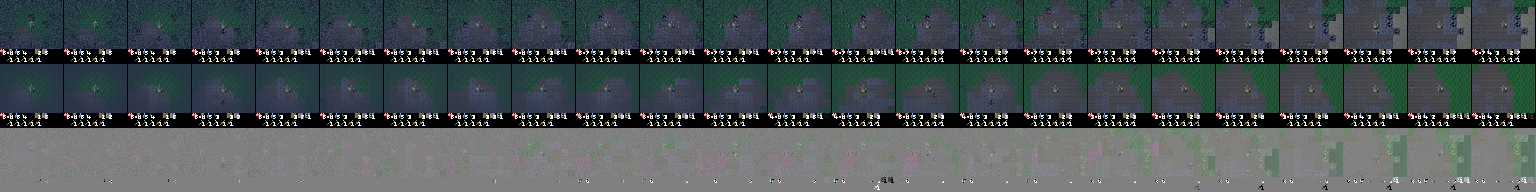
\includegraphics[width=\linewidth]{field-open-loop-station-inside.png}
  \caption{Open-loop prediction from the beside-resource anchored run at 100k steps. Rows: environment frames, model frames (the first eight columns reconstruct from the posterior, the rest are imagined from the prior given the recorded actions), and absolute error. The segment is the probe window with the most station cells; the environment frames themselves are dark, as at night in Crafter's day cycle. The other two runs give visually similar strips. We report the field head, not these images.}
  \label{fig:openloop}
\end{figure}

\section{Reproducibility}
\label{app:repro}

Every number, table, and plot in this paper is produced from the training logs and probe summaries by one script, which reads the per-life and per-episode logs, applies the exclusion rule of \cref{app:inject}, recounts the actor's and demonstrator's lives, and writes the tables and figures.
\Cref{fig:example} comes from a separate inference-only script that runs one benchmark checkpoint over a stored probe episode, and the injection leak is reproduced by a script that uses the environment alone.
The repository contains the world model, the field head, the room environment and demonstrator, the training loops for both settings, the probe scripts, and the configuration files for all seven runs.
At the logged rate of 0.65--1.05 environment steps per second, a benchmark run took one to two days on one 16\,GB GPU; a room run took under an hour.
